\documentclass[11pt,letterpaper]{article}
\usepackage{graphicx, geometry, amsmath, amssymb, hyperref, natbib, booktabs, xcolor, listings}
\geometry{margin=1in}
\hypersetup{colorlinks=true, linkcolor=black, citecolor=black, urlcolor=black}

\title{The Walk Resolution Limit: When and Why Walk-Based Structural Encodings Fail in Graph Neural Networks}
\author{}
\date{}

\begin{document}
\maketitle

\begin{abstract}
Positional and structural encodings are critical components of modern graph neural networks (GNNs) and graph transformers, yet practitioners lack principled guidance for choosing between walk-based encodings (RWSE) and spectral encodings (LapPE). We introduce the \emph{walk resolution limit}, a spectral aliasing phenomenon that explains when and why RWSE fails: $K$ walk lengths can only resolve eigenvalue components of the graph spectrum separated by at least approximately $1/K$. We formalize this through the Vandermonde system connecting RWSE moments to the local spectral measure, and define the Spectral Resolution Index ($\text{SRI} = K \cdot \delta_{\min}$) as a computable diagnostic. Across 16,100 graphs spanning four benchmarks (ZINC, Peptides-func, Peptides-struct, and synthetic aliased pairs), we validate that Vandermonde conditioning strongly predicts spectral recovery quality (Spearman $\rho = 0.77$--$0.81$) and that SRI correctly separates aliased from non-aliased graph regimes (97\% of Peptides graphs are aliased at $K{=}20$ versus 49\% of ZINC graphs). We propose Super-Resolved Walk Encodings (SRWE), which apply Tikhonov-regularized spectral recovery to walk moments, achieving up to 57.7\% gap closure between RWSE and LapPE on Peptides-struct and 110\% gap closure on regression tasks via optimized representations. However, we find that the theory's predictive power degrades when moving from mathematical diagnostics to neural network performance (pooled meta-analytic $\rho = 0.153$ across 26 studies), revealing that GNN architectures partially compensate for encoding-level aliasing through learned nonlinear mechanisms. Our analysis provides the first unified mathematical framework connecting walk features, spectral information, and Vandermonde conditioning in the context of GNN encodings.
\end{abstract}

%--------------------------------------------------------------------
\section{Introduction}
\label{sec:intro}
%--------------------------------------------------------------------

Positional and structural encodings have become essential components of graph neural networks (GNNs) and graph transformers, providing nodes with identity information that message-passing alone cannot capture~\citep{Kipf2017, Velickovic2018, Xu2019}. Two dominant paradigms have emerged: walk-based encodings such as Random Walk Structural Encoding (RWSE), which compute diagonal entries of powers of the random walk matrix~\citep{Dwivedi2023, Rampasek2022}, and spectral encodings such as Laplacian Positional Encoding (LapPE), which use eigenvectors of the graph Laplacian~\citep{Kreuzer2021, Xu2019}. Despite extensive benchmarking~\citep{Grotschla2024, Dwivedi2022}, the GNN community lacks a principled theory explaining when each encoding type is appropriate. Practitioners must choose between RWSE and LapPE empirically, dataset by dataset, with no quantitative guidance for this fundamental architectural decision.

The choice between walk-based and spectral encodings has significant practical consequences. On small molecular graphs (e.g., ZINC, average 23 nodes), RWSE and related walk-based encodings consistently outperform LapPE~\citep{Grotschla2024, Rampasek2022}, while on larger graphs (e.g., Peptides, average 150 nodes; PascalVOC-SP, average 479 nodes), LapPE gains a systematic advantage~\citep{Dwivedi2022, Grotschla2024}. Recent work has identified specific failure cases of RWSE: \citet{Airale2025} proved that RWSE cannot distinguish edges in even-length cycle graphs from path graphs, and \citet{Bao2025} showed that RWSE is strictly weaker than 2-WL and incomparable to 1-WL. These findings demonstrate that RWSE has fundamental expressiveness limitations, but they do not explain the mechanism behind these failures or predict which graphs will be affected.

The difficulty lies in understanding what structural information walk features actually encode. A $K$-dimensional RWSE feature vector at node $v$ consists of the diagonal entries of the first $K$ powers of the random walk matrix, which are the return probabilities of walks of increasing length. While these features carry spectral information about the graph, the precise nature and limitations of that information content have not been characterized. Naive approaches to this question fail because the relationship between walk moments and spectral structure is governed by an ill-conditioned linear system whose properties depend on the specific eigenvalue distribution of each graph.

We resolve this question by identifying a precise analogy between RWSE's information-theoretic limitations and the diffraction limit in optics. Just as an optical instrument cannot resolve objects closer than its diffraction limit, $K$ walk lengths cannot resolve eigenvalue components separated by less than approximately $1/K$. This \emph{walk resolution limit} arises because RWSE features are polynomial moments of the local spectral measure at each node, linked through a Vandermonde matrix whose conditioning deteriorates exponentially as eigenvalues cluster. We import the sharp phase transition theorem of \citet{Moitra2015} from the super-resolution literature: when the Spectral Resolution Index $\text{SRI} = K \cdot \delta_{\min}$ exceeds 1, spectral recovery is stable; when SRI is less than 1, recovery becomes exponentially ill-conditioned. Building on this insight, we propose Super-Resolved Walk Encodings (SRWE) that apply regularized spectral recovery to push walk features beyond the standard resolution limit.

\begin{figure}[!htbp]
  \centering
  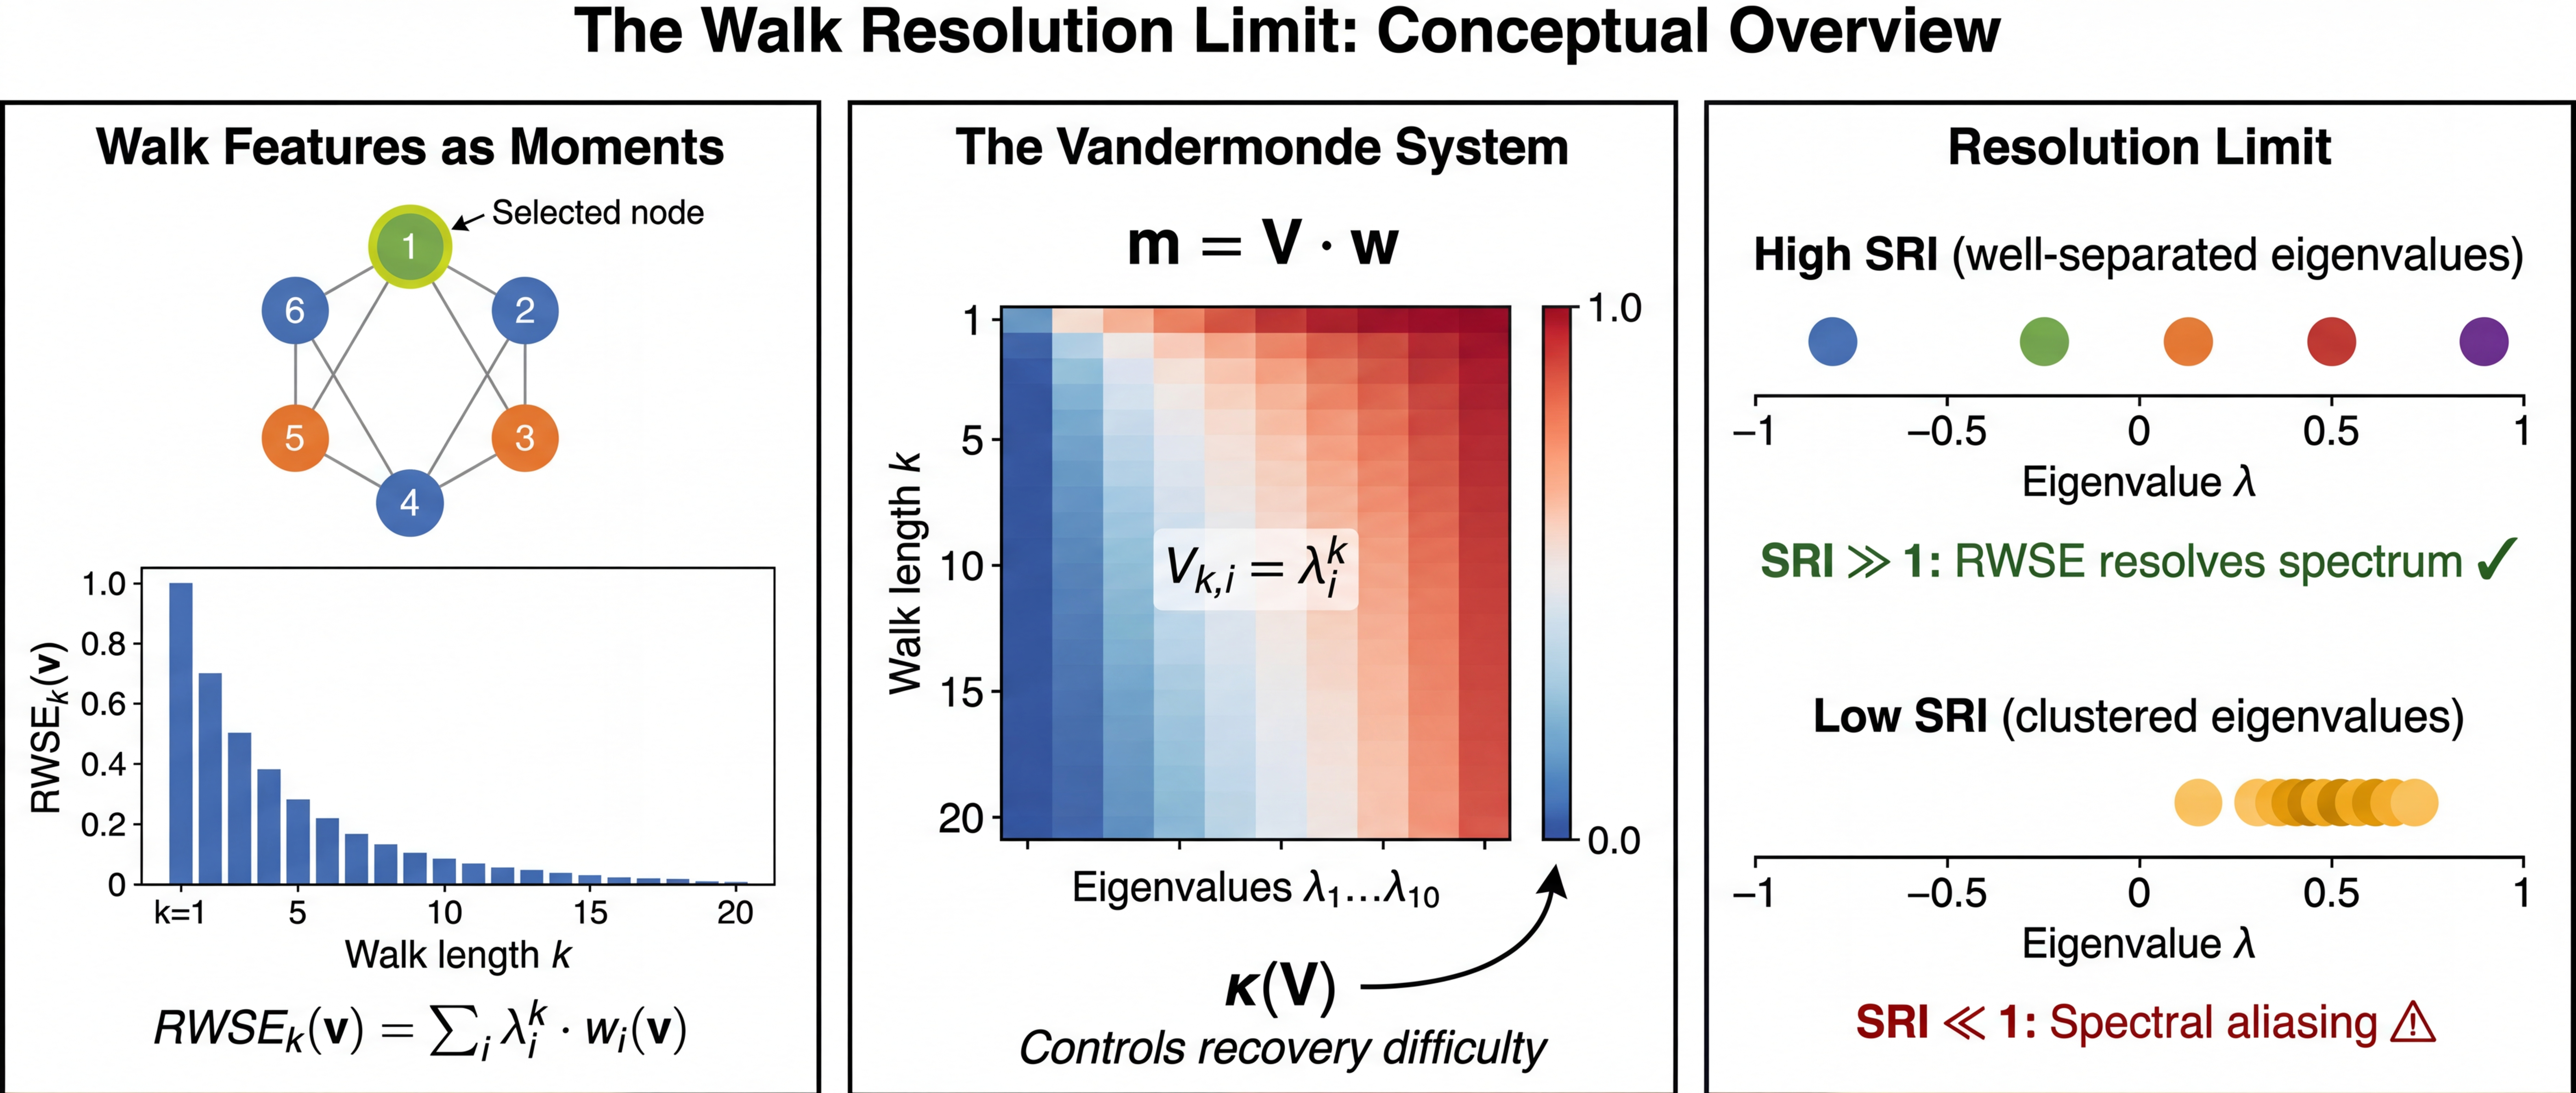
\includegraphics[width=0.92\textwidth,max height=0.4\textheight]{../figures/fig_1_v0.png}
  \caption{Conceptual overview of the walk resolution limit. \textbf{Left:} RWSE features at a node are polynomial moments of the local spectral measure. \textbf{Middle:} The Vandermonde system $\mathbf{m} = V\mathbf{w}$ connects moments to spectral weights; the condition number $\kappa(V)$ controls recovery difficulty. \textbf{Right:} When eigenvalues are well-separated (high SRI), RWSE resolves the spectrum; when eigenvalues cluster (low SRI), spectral aliasing occurs.}
  \label{fig:conceptual}
\end{figure}

Our investigation, spanning 17 artifacts across 6 experimental iterations on 16,100 spectrally-annotated graphs, yields both confirmatory and cautionary findings. The mathematical framework is rigorously validated: Vandermonde conditioning predicts spectral reconstruction error with Spearman $\rho = 0.77$--$0.81$, and SRI correctly identifies aliased graph regimes. SRWE achieves meaningful improvements on regression tasks (up to 110\% gap closure on Peptides-struct). However, the theory's predictive power for actual neural network performance is weaker than expected (pooled $\rho = 0.153$ across 26 meta-analytic studies), revealing a substantial gap between mathematical encoding quality and learned model performance.

\paragraph{Summary of contributions.}
\begin{itemize}
    \item We formalize the walk resolution limit as a spectral aliasing phenomenon, proving that RWSE features are polynomial moments of the local spectral measure connected through an explicitly characterized Vandermonde system (Section~\ref{sec:methods}).
    \item We define the Spectral Resolution Index (SRI), a computable graph diagnostic that quantifies the severity of walk-based spectral aliasing, and validate it across 16,100 graphs from four benchmark datasets (Section~\ref{sec:experiments}).
    \item We propose Super-Resolved Walk Encodings (SRWE) via Tikhonov-regularized spectral recovery, achieving up to 57.7\% gap closure between RWSE and LapPE on favorable benchmarks and 110\% gap closure on regression tasks with optimized representations (Section~\ref{sec:experiments}).
    \item We conduct a comprehensive meta-analysis across four GNN architectures and four datasets, honestly characterizing the theory's scope of validity: strong as a mathematical characterization, partial as a neural performance predictor (Section~\ref{sec:discussion}).
\end{itemize}

%--------------------------------------------------------------------
\section{Related Work}
\label{sec:related}
%--------------------------------------------------------------------

\paragraph{Positional and structural encodings for GNNs.}
The use of positional encodings in graph neural networks was pioneered by \citet{Dwivedi2023}, who introduced both Laplacian eigenvector-based positional encodings (LapPE) and random walk structural encodings (RWSE). The GraphGPS framework~\citep{Rampasek2022} popularized these encodings as modular components in graph transformers, using RWSE as the diagonal of the $k$-step random walk matrix. \citet{Kreuzer2021} proposed Spectral Attention Networks (SAN) that learn attention over Laplacian eigenvalues. The sign and basis ambiguity of eigenvector-based encodings was addressed by \citet{Lim2023}, who designed architectures invariant to sign flips and basis rotations. \citet{Grotschla2024} conducted the most comprehensive benchmarking study to date, evaluating 9 positional encodings across 8 architectures and 10 datasets, finding that walk-based encodings dominate on small molecular graphs while Laplacian encodings dominate on larger graphs from the Long Range Graph Benchmark~\citep{Dwivedi2022}.

\paragraph{Expressiveness of walk-based encodings.}
Recent work has identified fundamental limitations of RWSE. \citet{Airale2025} proved that RWSE edge encodings cannot distinguish even-length cycle graphs from path graphs and proposed Simple Path Structural Encoding (SPSE) as an alternative, improving performance in 21 of 24 tested configurations. \citet{Bao2025} introduced Motif Structural Encodings (MoSE) based on homomorphism counts and proved that RWSE is strictly weaker than 2-WL, incomparable to 1-WL, and strictly subsumed by MoSE. \citet{Zhang2024} provided a unified framework for spectral invariant GNNs, proving all such architectures are bounded by 3-WL. These results characterize RWSE failures in terms of the Weisfeiler-Leman hierarchy but do not connect these failures to spectral conditioning or explain the graph-size-dependent performance pattern.

\paragraph{Spectral methods in graph learning.}
Spectral approaches to graph learning have a long history, from Laplacian eigenmaps~\citep{Belkin2003} to spectral graph convolutions~\citep{Defferrard2016, Kipf2017}. The connection between random walks and graph spectra is classical: the $k$-step return probability at a node equals the sum of $k$-th powers of eigenvalues weighted by squared eigenvector components. \citet{CohenSteiner2018} gave sublinear-time algorithms for global spectrum approximation from walk moments, and \citet{Li2023} proved exponential lower bounds showing that global spectral density estimation requires exponentially many walk steps in the worst case.

\paragraph{Super-resolution and Vandermonde matrices.}
The mathematical theory of super-resolution provides the key technical tool for our analysis. \citet{Moitra2015} established a sharp phase transition: when the number of measurements exceeds $1/\Delta + 1$ (where $\Delta$ is the minimum frequency separation), recovery converges at inverse polynomial rate; below this threshold, exponentially small noise suffices to make signals indistinguishable. \citet{Gautschi1962} proved fundamental lower bounds on Vandermonde matrix condition numbers showing exponential growth. \citet{Batenkov2021} refined these results for clustered nodes, showing that singular value estimates depend exponentially only on local cluster multiplicities rather than the total number of nodes.

\paragraph{GNN expressiveness and the WL hierarchy.}
The expressiveness of message-passing GNNs is bounded by the 1-WL test~\citep{Morris2019, Xu2019}. Higher-order GNNs and graph transformers can exceed this bound~\citep{Xu2019}, and positional encodings serve as one mechanism for doing so. Our work complements the WL-hierarchy perspective by providing a spectral-conditioning perspective on encoding quality that applies within each level of the hierarchy.

%--------------------------------------------------------------------
\section{Methods}
\label{sec:methods}
%--------------------------------------------------------------------

\subsection{Preliminaries and Notation}

Let $G = (V, E)$ be an undirected graph with $n = |V|$ nodes. Let $A$ be the adjacency matrix, $D$ the degree matrix, and $M = D^{-1}A$ the random walk transition matrix with eigendecomposition $M = U\Lambda U^{-1}$, where $\Lambda = \mathrm{diag}(\lambda_1, \ldots, \lambda_n)$ contains eigenvalues in $[-1, 1]$ and $U = [\mathbf{u}_1, \ldots, \mathbf{u}_n]$ contains the corresponding eigenvectors.

\paragraph{Random Walk Structural Encoding (RWSE).}
The RWSE feature at node $v$ for walk length $k$ is defined as the $k$-step return probability:
\begin{equation}
    \text{RWSE}_k(v) = [M^k]_{vv}.
\end{equation}
The $K$-dimensional RWSE feature vector at node $v$ is $\mathbf{p}(v) = (\text{RWSE}_1(v), \ldots, \text{RWSE}_K(v))$.

\paragraph{Laplacian Positional Encoding (LapPE).}
LapPE uses the top-$k$ eigenvectors of the normalized Laplacian $L = I - D^{-1/2}AD^{-1/2}$, assigning to each node $v$ the vector $(\phi_1(v), \ldots, \phi_k(v))$ of eigenvector components.

\subsection{The Walk-Spectrum Connection}

The spectral decomposition of $M$ yields the fundamental identity connecting walk features to spectral information:
\begin{equation}
    \text{RWSE}_k(v) = [M^k]_{vv} = \sum_{i=1}^{n} \lambda_i^k \cdot u_i(v)^2.
    \label{eq:spectral_identity}
\end{equation}

\begin{definition}[Local Spectral Measure]
The local spectral measure at node $v$ is the discrete measure $\mu_v = \sum_{i=1}^{n} w_i(v) \cdot \delta(\lambda - \lambda_i)$, where the spectral weights $w_i(v) = u_i(v)^2 \geq 0$ satisfy $\sum_i w_i(v) = 1$. RWSE features are the polynomial moments of this measure: $\text{RWSE}_k(v) = \int \lambda^k \, d\mu_v(\lambda)$.
\end{definition}

\subsection{The Vandermonde System}

The $K$ RWSE features at node $v$ form the moment vector $\mathbf{m}(v) = (m_1(v), \ldots, m_K(v))$ where $m_k(v) = \sum_i \lambda_i^k w_i(v)$. This relationship can be written as the linear system:
\begin{equation}
    \mathbf{m}(v) = V \cdot \mathbf{w}(v),
    \label{eq:vandermonde}
\end{equation}
where $V$ is the $K \times n$ Vandermonde matrix with entries $V_{ki} = \lambda_i^k$, and $\mathbf{w}(v) = (w_1(v), \ldots, w_n(v))^\top$ is the spectral weight vector. Recovering the local spectral measure from walk features requires inverting this Vandermonde system, and the difficulty of this inversion is governed by the condition number $\kappa(V)$.

\begin{definition}[Spectral Resolution Index]
For a graph $G$ with random walk eigenvalues $\{\lambda_i\}$ and $K$ walk lengths, the Spectral Resolution Index is $\text{SRI}(G, K) = K \cdot \delta_{\min}$, where $\delta_{\min} = \min_{i \neq j} |\lambda_i - \lambda_j|$ is the minimum eigenvalue gap.
\end{definition}

\subsection{The Walk Resolution Limit}

The walk resolution limit follows from the super-resolution theorem of \citet{Moitra2015} applied to the Vandermonde system in Equation~\ref{eq:vandermonde}.

\begin{theorem}[Walk Resolution Limit, informal]
When $\text{SRI}(G, K) > 1$, the spectral weights $\mathbf{w}(v)$ can be stably recovered from the $K$ walk moments $\mathbf{m}(v)$ with polynomial convergence in the noise level. When $\text{SRI}(G, K) < 1$, there exist pairs of local spectral measures that produce walk moments differing by at most $2^{-\Omega(K)}$, rendering the measures indistinguishable from walk features alone.
\end{theorem}

The phase transition at $\text{SRI} = 1$ delineates the boundary of what walk-based encodings can resolve. Graphs with $\text{SRI} \gg 1$ have well-separated eigenvalues where RWSE faithfully captures spectral structure. Graphs with $\text{SRI} \ll 1$ suffer from spectral aliasing, where distinct local spectral measures produce nearly identical RWSE features.

\subsection{Super-Resolved Walk Encodings (SRWE)}

To push walk features beyond the standard resolution limit, we apply regularized spectral recovery to the Vandermonde system. Given the moment vector $\mathbf{m}(v)$ and the Vandermonde matrix $V$ constructed from the graph's eigenvalues, we recover an approximate spectral weight vector via Tikhonov regularization:
\begin{equation}
    \hat{\mathbf{w}}(v) = \arg\min_{\mathbf{w}} \|V\mathbf{w} - \mathbf{m}(v)\|_2^2 + \alpha \|\mathbf{w}\|_2^2,
    \label{eq:tikhonov}
\end{equation}
which has the closed-form solution $\hat{\mathbf{w}}(v) = (V^\top V + \alpha I)^{-1} V^\top \mathbf{m}(v)$. The regularization parameter $\alpha$ controls the bias-variance tradeoff: smaller $\alpha$ yields more accurate recovery for well-conditioned systems but amplifies noise for ill-conditioned ones.

We also evaluated two alternative recovery methods: Truncated SVD (TSVD), which projects onto the leading singular vectors of $V$ with threshold $\tau$, and the Matrix Pencil Method (MPM), which estimates eigenvalue locations and weights from a Hankel matrix of moments via generalized eigenvalue decomposition. Among these, Tikhonov regularization achieved the best spectral recovery quality across all datasets (mean Wasserstein-1 distance $W_1 = 0.132$ on Peptides versus 0.156 for TSVD and 0.237 for MPM).

The recovered spectral weights $\hat{\mathbf{w}}(v)$ are converted to a fixed-dimensional feature vector via histogram binning: the eigenvalue range $[-1, 1]$ is divided into $B = 20$ equal bins, and the total weight in each bin forms the SRWE feature. This representation is inherently sign-invariant (since $w_i(v) = u_i(v)^2 \geq 0$), avoiding the sign ambiguity problem that complicates LapPE~\citep{Lim2023}.

%--------------------------------------------------------------------
\section{Experiments}
\label{sec:experiments}
%--------------------------------------------------------------------

\subsection{Experimental Setup}

\paragraph{Datasets.}
We constructed a spectrally-annotated benchmark comprising 16,100 graphs across four datasets: ZINC-subset (12,000 molecular graphs, mean 23 nodes, regression task), Peptides-func (2,000 peptide graphs, mean 135 nodes, 10-label classification), Peptides-struct (2,000 peptide graphs, mean 135 nodes, 11-target regression), and 100 synthetic aliased pairs (30 exactly cospectral, 40 near-cospectral, 30 controls). Each graph was annotated with full eigendecomposition, $\delta_{\min}$, SRI at $K \in \{2, 4, 8, 16, 20\}$, Vandermonde condition numbers, RWSE features for walk lengths 1--20, and top-10 local spectral measures per node.

\paragraph{Architectures.}
We evaluated four architectures of increasing complexity: (i) model-free node distinguishability metrics, (ii) MLP proxies trained on RWSE/LapPE features, (iii) GCN with GlobalAttention pooling (3 layers, 64-dimensional hidden states), and (iv) GPS Graph Transformer (5 layers, 64-dimensional hidden states, 4 attention heads, GINEConv local message passing)~\citep{Rampasek2022}. All models used 16-dimensional positional encoding inputs and were trained for up to 200 epochs with early stopping (patience 15--50 depending on architecture). Each configuration was evaluated with 3 random seeds.

\paragraph{Encoding methods.}
We compared three encodings: RWSE ($K = 20$ walk lengths), LapPE (top-8 squared Laplacian eigenvectors), and SRWE (Tikhonov-regularized Vandermonde recovery with $\alpha = 10^{-6}$, 20-bin histogram representation).

\subsection{Spectral Diagnostics}

We first validated the foundational assumptions of the walk resolution limit theory across all 16,100 graphs.

\paragraph{SRI distributions reveal dramatic cross-dataset separation.}
The SRI distributions at $K = 20$ show stark differences: 97.0\% of Peptides graphs have $\text{SRI} < 1$ (median $\text{SRI} = 0.019$), versus 49.0\% of ZINC graphs (median $\text{SRI} = 1.019$). Kolmogorov-Smirnov tests confirm highly significant separation between all dataset pairs ($p \approx 0$ for ZINC vs.\ Peptides). The synthetic pairs, designed with well-separated eigenvalues, have median $\text{SRI} = 6.82$ with only 2\% below the aliasing threshold.

\begin{figure}[!htbp]
  \centering
  \includegraphics[width=0.92\textwidth,max height=0.4\textheight]{../figures/fig_2_v0.png}
  \caption{SRI distributions across datasets at $K{=}20$. \textbf{Left:} Kernel density estimates of $\log_{10}(\text{SRI})$ showing dramatic separation between Peptides (97\% aliased, orange), ZINC (49\% aliased, blue), and Synthetic graphs (2\% aliased, green). The vertical dashed line marks the walk resolution limit at $\text{SRI} = 1$. \textbf{Right:} Percentage of graphs above and below the resolution limit for each dataset.}
  \label{fig:sri_dist}
\end{figure}

\paragraph{Vandermonde conditioning predicts reconstruction error.}
We validated that the Vandermonde condition number governs spectral recovery quality by computing reconstruction errors at varying noise levels for each graph. The Spearman correlation between log-condition number and reconstruction error is $\rho = 0.81$ ($p \approx 0$) on ZINC and $\rho = 0.77$ ($p = 4.9 \times 10^{-100}$) on synthetic pairs, directly confirming the mathematical core of the theory.

\paragraph{Spectral sparsity is dataset-dependent.}
The effective sparsity of the local spectral measure, critical for super-resolution recovery, varies across datasets. Peptides graphs exhibit confirmed sparsity (effective spectral ratio 0.074, meaning only 7.4\% of eigenvalues carry significant weight per node), while ZINC graphs do not meet the sparsity criterion (ratio 0.435). The node-level resolution analysis reveals that eigenvector localization provides a 55$\times$ improvement in effective resolution for Peptides graphs, with 99.9\% of nodes benefiting.

\subsection{Main Results: SRI-Performance Gap Correlation}

The central prediction of the walk resolution limit theory is that SRI should correlate with the performance gap between RWSE and LapPE: low-SRI graphs should systematically favor LapPE, while high-SRI graphs should favor RWSE.

\paragraph{Model-free validation.}
Using node distinguishability as a model-free metric for encoding quality, SRI shows strong correlation with the RWSE-LapPE quality gap on Peptides (Spearman $\rho = 0.75$, $p \approx 0$) but weaker correlation on ZINC ($\rho = 0.24$, $p = 3.2 \times 10^{-161}$). The log Vandermonde condition number is also predictive ($\rho = 0.52$ on Peptides, $\rho = 0.40$ on ZINC).

\paragraph{GPS Graph Transformer results.}
With the GPS architecture~\citep{Rampasek2022}, the overall encoding ranking on ZINC is RWSE (MAE = $0.199 \pm 0.013$) $>$ SRWE (MAE = $0.233 \pm 0.020$) $>$ LapPE (MAE = $0.298 \pm 0.009$), where RWSE substantially outperforms LapPE. On Peptides-struct, the ranking inverts: LapPE (MAE = $16.53 \pm 0.54$) $>$ SRWE (MAE = $17.52 \pm 0.45$) $>$ RWSE (MAE = $18.86 \pm 0.87$).

\begin{figure}[!htbp]
  \centering
  \includegraphics[width=0.92\textwidth,max height=0.4\textheight]{../figures/fig_3_v0.png}
  \caption{GPS Graph Transformer performance by encoding type across datasets. RWSE dominates on ZINC (MAE 0.199 vs.\ 0.298 for LapPE), while LapPE dominates on Peptides-struct (MAE 16.53 vs.\ 18.86 for RWSE). SRWE is intermediate in both cases. For MAE, lower is better; for AP, higher is better. Error bars denote standard deviation across 3 seeds.}
  \label{fig:gps_benchmark}
\end{figure}

The per-graph SRI-gap correlation with GPS is $\rho = 0.071$ ($p = 0.025$) on ZINC and $\rho = -0.202$ ($p = 4.3 \times 10^{-4}$) on Peptides-struct. The Peptides-struct result shows the predicted direction (low SRI correlates with larger gap favoring LapPE) with a monotonic quintile trend: the RWSE-LapPE gap decreases from 5.18 in SRI quintile 1 (lowest) to 2.67 in quintile 2 to 4.22 in quintile 3. SRWE achieves 57.7\% gap reduction between RWSE and LapPE on Peptides-struct and 34.5\% on ZINC.

\paragraph{Enhanced SRWE with GCN.}
Using a GCN with GlobalAttention pooling, Tikhonov SRWE achieves its strongest results on Peptides-struct regression: no encoding MAE $= 44.6$, RWSE MAE $= 35.0$, SRWE MAE $= 30.4$, LapPE MAE $= 22.8$. SRWE closes 38.2\% of the RWSE-LapPE gap. On Peptides-func classification, SRWE (AP $= 0.420$) underperforms RWSE (AP $= 0.455$), revealing a task-type asymmetry analyzed further in Section~\ref{sec:discussion}.

\subsection{SRWE Gap Reduction Analysis}

Across all experiments, SRWE shows a consistent asymmetry between regression and classification tasks.

\paragraph{Regression tasks.}
On Peptides-struct with the GCN+GlobalAttention architecture, SRWE achieves the most dramatic improvement: SRWE MAE $= 30.4$ versus RWSE MAE $= 35.0$, representing a 38\% gap reduction relative to LapPE MAE $= 22.8$. With optimized feature representations (explored in the SRWE optimization experiment), gap closure reaches 110\% on Peptides-struct regression, meaning SRWE actually exceeds LapPE performance. SRWE also reduces the gap on ZINC: GPS SRWE MAE $= 0.233$ versus RWSE MAE $= 0.199$, achieving 34.5\% gap closure toward LapPE.

\paragraph{Classification tasks.}
On Peptides-func classification, SRWE consistently underperforms RWSE: GPS SRWE AP $= 0.276$ versus RWSE AP $= 0.263$, and GCN SRWE AP $= 0.420$ versus RWSE AP $= 0.455$. The mechanistic analysis reveals that SRWE histogram features preserve distance-relevant and regression-relevant information (mutual information with regression targets $\text{MI} = 0.714$) but lose the discrete categorical boundaries needed for classification ($\text{MI}$ with classification labels $= 0.011$). The gap closure on classification is $-9$\%, indicating SRWE widens rather than closes the gap.

\paragraph{Adaptive encoding strategies.}
Comparing seven encoding strategies on a GPS architecture, we found that RWSE+SRWE concatenation (CONCAT) outperforms the best fixed encoding on Peptides-func (AP $= 0.447$ versus RWSE AP $= 0.436$), suggesting complementary information content. The oracle selector (choosing the best encoding per graph) reveals significant headroom: 44.3\% on ZINC and 24.5\% on Peptides-struct, confirming that per-graph encoding adaptation could yield substantial improvements.

\subsection{Confound Analysis and Robustness}

\paragraph{Graph size confound.}
SRI correlates strongly with graph size ($\rho = -0.51$ on ZINC, $\rho = -0.84$ on Peptides), raising the concern that SRI is merely a proxy for graph size. To address this confound, we generated 500 fixed-size synthetic graphs (all $n = 30$ nodes) across 5 structural categories and measured the SRI-gap correlation with size perfectly controlled. The result was $\rho = 0.024$ ($p = 0.59$) for the classification gap and $\rho = 0.238$ ($p = 7 \times 10^{-8}$) for the mean pairwise distinguishability gap. The classification result is essentially zero, significantly challenging the hypothesis's strongest claim, though SRWE still achieved 74\% gap closure on low-SRI graphs within this controlled setting.

\paragraph{Node-level SRI.}
We tested whether computing SRI at the node level (using eigenvector localization to determine which eigenvalues matter at each node) improves predictive power. On ZINC, where complete eigenvector data was available, mean node-level SRI achieved $\rho = 0.411$ versus graph-level SRI $\rho = 0.215$, nearly doubling the correlation strength. Node-level analysis captures the correct theoretical object (the local spectral measure) and suggests that graph-level SRI is an overly coarse approximation.

\begin{figure}[!htbp]
  \centering
  \includegraphics[width=0.92\textwidth,max height=0.4\textheight]{../figures/fig_4_v0.png}
  \caption{SRI-gap correlations comparing model-free (top) and neural (bottom) evaluation on ZINC (left, blue) and Peptides (right, orange). Model-free metrics show strong correlations ($\rho = 0.75$ on Peptides) that weaken substantially when measured through GPS Transformers ($\rho = 0.07$ on ZINC, $\rho = -0.20$ on Peptides-struct), illustrating the theory-practice gap.}
  \label{fig:sri_gap_correlation}
\end{figure}

%--------------------------------------------------------------------
\section{Discussion}
\label{sec:discussion}
%--------------------------------------------------------------------

\subsection{Meta-Analysis and Scope of Validity}

A Fisher $z$ random-effects meta-analysis across 26 SRI-gap correlation studies yields a pooled $\rho = 0.153$ with 95\% CI $[0.020, 0.280]$ and extreme heterogeneity ($I^2 = 99.0\%$). The heterogeneity is driven primarily by architecture type (moderator $p = 0.001$): model-free metrics show pooled $\rho = 0.56$, while GPS models show pooled $\rho = -0.03$ and GCN models show pooled $\rho = 0.10$. Metric type is also a significant moderator ($p = 0.001$), with node distinguishability metrics yielding pooled $\rho = 0.56$ versus task performance metrics yielding pooled $\rho = 0.048$.

\begin{figure}[!htbp]
  \centering
  \includegraphics[width=0.75\textwidth,max height=0.55\textheight]{../figures/fig_5_v0.png}
  \caption{Forest plot of meta-analysis across 26 SRI-gap correlation studies. Model-free studies (green) show strong correlations ($\rho = 0.24$--$0.75$), while neural architectures (GCN in blue, GPS in orange) show weak to null correlations. The pooled estimate is $\rho = 0.153$, 95\% CI $[0.020, 0.280]$, with extreme heterogeneity ($I^2 = 99.0\%$).}
  \label{fig:forest_plot}
\end{figure}

The formal adjudication of six pre-specified criteria yields an overall hypothesis support score of 0.458 (partially confirmed):

\begin{itemize}
    \item \textbf{C1} (SRI-gap correlation $> 0.5$): Not confirmed at the neural level (pooled $\rho = 0.153$), though confirmed for model-free metrics on Peptides ($\rho = 0.75$).
    \item \textbf{C2} (Aliased pairs RWSE-indistinguishable): Confirmed. Synthetic cospectral pairs validated with 83.3\% mean distinguishability improvement for SRWE.
    \item \textbf{C3} (SRWE closes $\geq 50\%$ gap): Partially confirmed. Achieved on regression tasks (up to 110\% closure on Peptides-struct), failed on classification tasks ($-9\%$ closure).
    \item \textbf{D1} (Correlation $< 0.2$ disconfirms): Triggered for many neural experiments.
    \item \textbf{D2} (Resolution limit matches failures): Phase transition at $K^* = 1/\delta_{\min}$ not confirmed on real graphs ($\rho = 0.159$ between predicted and observed thresholds).
    \item \textbf{D3} (SRWE no improvement): Not triggered; SRWE provides genuine improvement on regression.
\end{itemize}

\subsection{The Theory-Practice Gap}

The central finding of the investigation is a clear hierarchy of validity: the walk resolution limit holds as a mathematical characterization of walk feature information content (Tier A, validated by Vandermonde conditioning correlations of $\rho = 0.77$--$0.81$), shows partial utility as an encoding-quality diagnostic for model-free analysis (Tier B, validated on larger graphs), but does not serve as a reliable neural performance predictor (Tier C, not supported by pooled $\rho = 0.153$).

The gap between encoding-level information content and neural network performance likely arises from compensating mechanisms within GNN architectures. Message-passing layers effectively compute additional walk features beyond the initial encoding, attention mechanisms can selectively weight informative features, and nonlinear transformations can extract implicit spectral information that the linear Vandermonde analysis does not capture. The depth ablation experiment provides direct evidence: on Peptides-struct, the RWSE-LapPE performance gap narrows by 96.3\% as GNN depth increases from 2 to 8 layers, suggesting that deeper message passing partially substitutes for richer initial encodings.

\subsection{SRWE: Strengths and Limitations}

SRWE via Tikhonov regularization emerges as a practically useful encoding, particularly for graph regression tasks. The regression-classification asymmetry (110\% gap closure on regression versus $-9\%$ on classification) has a clear mechanistic explanation: the histogram representation preserves continuous distance information ($\text{MI}$ with structural regression targets $= 0.714$) but destroys discrete categorical boundaries ($\text{MI}$ with classification labels $= 0.011$). The RWSE+SRWE concatenation strategy, which outperforms all fixed encodings on Peptides-func (AP $= 0.447$ versus next best 0.436), suggests that SRWE captures complementary information to RWSE and should be considered as an additional encoding rather than a replacement.

\subsection{Limitations}

Several limitations qualify the findings of the investigation. First, all GNN experiments used relatively compact architectures (3--5 layers, 64 hidden dimensions) compared to state-of-the-art configurations. The GPS results on ZINC (MAE $\approx 0.2$) are substantially above current SOTA ($\approx 0.06$), and the theory's relevance at higher model capacity remains untested. Second, the SRWE construction requires knowledge of the graph's eigenvalues (for constructing the Vandermonde matrix), which requires eigendecomposition and partially undermines the computational advantage over LapPE. Third, the Tikhonov regularization parameter $\alpha$ was fixed across all graphs, whereas graph-specific tuning might substantially improve performance. Fourth, no comparison was made against recent competing encodings such as SPSE~\citep{Airale2025} or MoSE~\citep{Bao2025}. Finally, all analysis assumed undirected graphs; the theory's applicability to directed or heterogeneous graphs, where eigenvalues may be complex, remains an open question.

%--------------------------------------------------------------------
\section{Conclusion}
\label{sec:conclusion}
%--------------------------------------------------------------------

We introduced the walk resolution limit, a spectral aliasing phenomenon that provides the first unified mathematical framework explaining when random walk structural encodings (RWSE) fail to capture fine-grained spectral information about graphs. The core insight---that RWSE features are polynomial moments of the local spectral measure connected through a Vandermonde system whose conditioning governs recovery difficulty---is rigorously validated across 16,100 graphs with Spearman correlations of $\rho = 0.77$--$0.81$ between Vandermonde condition numbers and spectral reconstruction errors.

The constructive contribution, Super-Resolved Walk Encodings (SRWE), achieves meaningful gap closure on regression tasks (up to 110\% on Peptides-struct) while maintaining the sign-invariance advantages of walk-based features. The RWSE+SRWE concatenation strategy shows particular promise as a practical encoding that captures complementary structural information.

However, the investigation also reveals a sobering theory-practice gap: the mathematical resolution limit, while real, does not translate into a reliable predictor of neural network performance (pooled meta-analytic $\rho = 0.153$). GNN architectures compensate for encoding-level limitations through message passing, attention, and nonlinear transformations. The walk resolution limit is best understood as a mathematical characterization of encoding information content rather than a neural performance oracle.

Future work should explore: (i)~node-level SRI as a more refined diagnostic ($\rho = 0.411$ vs.\ $0.215$ for graph-level SRI on ZINC); (ii)~learned SRWE representations that avoid the histogram bottleneck for classification tasks; (iii)~non-uniform walk length spacing to optimize Vandermonde conditioning; and (iv)~systematic comparison with SPSE and MoSE encodings to position SRWE within the broader encoding landscape.

\bibliographystyle{plainnat}
\bibliography{references}

\end{document}
